\documentclass[a4paper,12pt]{article}
\usepackage[utf8]{inputenc}
\usepackage{amsmath, amssymb}
\usepackage{graphicx}
\usepackage{geometry}
\usepackage{fancyhdr}
\usepackage[hidelinks]{hyperref}
\usepackage[ngerman]{babel}
\usepackage{enumerate}
\usepackage{float}
\usepackage{longtable}
\usepackage{array}
\usepackage[table]{xcolor}
\usepackage{everypage}

\geometry{left=2.5cm, right=2.5cm, top=2.5cm, bottom=2.5cm}


\pagestyle{fancy}
\fancyhf{}
\fancyhead[L]{Gruppe 05}
\fancyhead[R]{\textbf{G}ame \textbf{D}esign \textbf{D}ocument}


\begin{document}
    \thispagestyle{plain}
    \begin{center}
        \large{\textbf{G}ame \textbf{D}esign \textbf{D}ocument} \\
    \end{center}
    \vspace{3em}
    \begin{center}
        \begin{figure}[h]
            \centering
            
\includegraphics[width=0.75\textwidth]{./figures/BreakingWorseLogo}
            \label{fig:Breaking Worse}
        \end{figure}
    \end{center}
    \vspace{1em}
    \begin{center}
        \textbf{Gruppe 05} \\
        \vspace{2em}
        Marlene Albrecht, Daniel Augustin, xxxxxx xxxxxxx,\\
        xxxxxx xxxxx, Taha Rezzoug, Matteo Wittenberg \\
        \vspace{1em}
        Tutor: Luis Schaffner
    \end{center}
    
    \vfill
    \begin{figure}[h]
        \centering
        
\includegraphics[width=0.2\textwidth]{./figures/uni-logo}
        \label{fig:uni-logo}
    \end{figure}
    \begin{center}
        Freiburg im Breisgau, 11.1.2025
    \end{center}

    \newpage
    \renewcommand{\contentsname}{Inhaltsverzeichnis}
    \tableofcontents

    \newpage
    \section{Änderungsliste}\label{sec:anderungsliste}
    Es wurde nichts grundlegendes an der Spieldefinition geändert, nur das GDD verbessert und Sachen besser definiert.

    \newpage
    \section{Spielkonzept}\label{sec:spielkonzept}
    Eine kurze, einleitende Zusammenfassung des Spiels und Beschreibung der zentralen Spielmechanik um einen Überblick über das Spiel zu bekommen.\\
    \subsection{Zusammenfassung}\label{subsec:zusammenfassung-des-spiels}

\begin{figure}[h]
    \centering
    \includegraphics[width=0.85\textwidth]{./figures/WaltUndJessie}
    \caption{Idealisierte Darstellung von den Spielfiguren Jesse und Walt.}
    \label{fig:figure}
\end{figure}

Ein Unglück kommt selten allein, du hast Krebs und die Heilung kostet ein Vermögen. 
Wo sollst du nur so schnell so viel Geld herbekommen? 
Zum Glück hat dein bester Freund eine Idee: Ihr steigt zusammen in das lokale Drogengeschäft ein. 
Mit einer Ausstattung, die noch sehr zu wünschen übriglässt und reichlich Motivation stürzt ihr euch ins Geschehen. 
Verborgen vor dem wachsamen Auge der Polizei und den immer gereizten Kräften des Organisierten Verbrechens müsst ihr die verschiedenen Gefahren und Herausforderungen des Drogengeschäfts meistern, bevor eure Zeit abläuft.
    \subsection{Zentrale Spielmechanik}\label{subsec:zentrale-spielmechanik}

Die beiden Spieler verbringen den Großteil ihrer Zeit damit, auf der begrenzten Stadtkarte genug Geld zu erwirtschaften um damit das gewinnbringende Item ,,Heilung'' zu kaufen, bevor ihnen die Zeit abläuft.
Dafür müssen sie Drogen in ihrem Haus aus verschiedenen, in der Stadt erworbenen, Rohstoffen herstellen und diese dann an neutrale NPCs verkaufen.
Dabei müssen sie darauf achten nicht von ihren Gegnern, Polizei und Kartell, entdeckt zu werden.
Hierfür müssen die Spieler vorausschauend Planen und die Risiken ihrer Gegner abwägen, um das Spiel zu gewinnen.


    \newpage
    \section{Benutzeroberfläche}\label{sec:benutzeroberflache}
    Hier wird erklärt, mit welchen Eingaben und über welche Steuerelemente der Spieler mit dem Spiel und dem Menü interagiert und wie diese aufgebaut sind.\\
    \subsection{Ingame Spieler Interface}\label{subsec:spieler-interface}

Bei \textbf{Breaking Worse} handelt es sich um ein 2D-Spiel mit Draufsicht: \\
\begin{figure}[h]
    \centering
    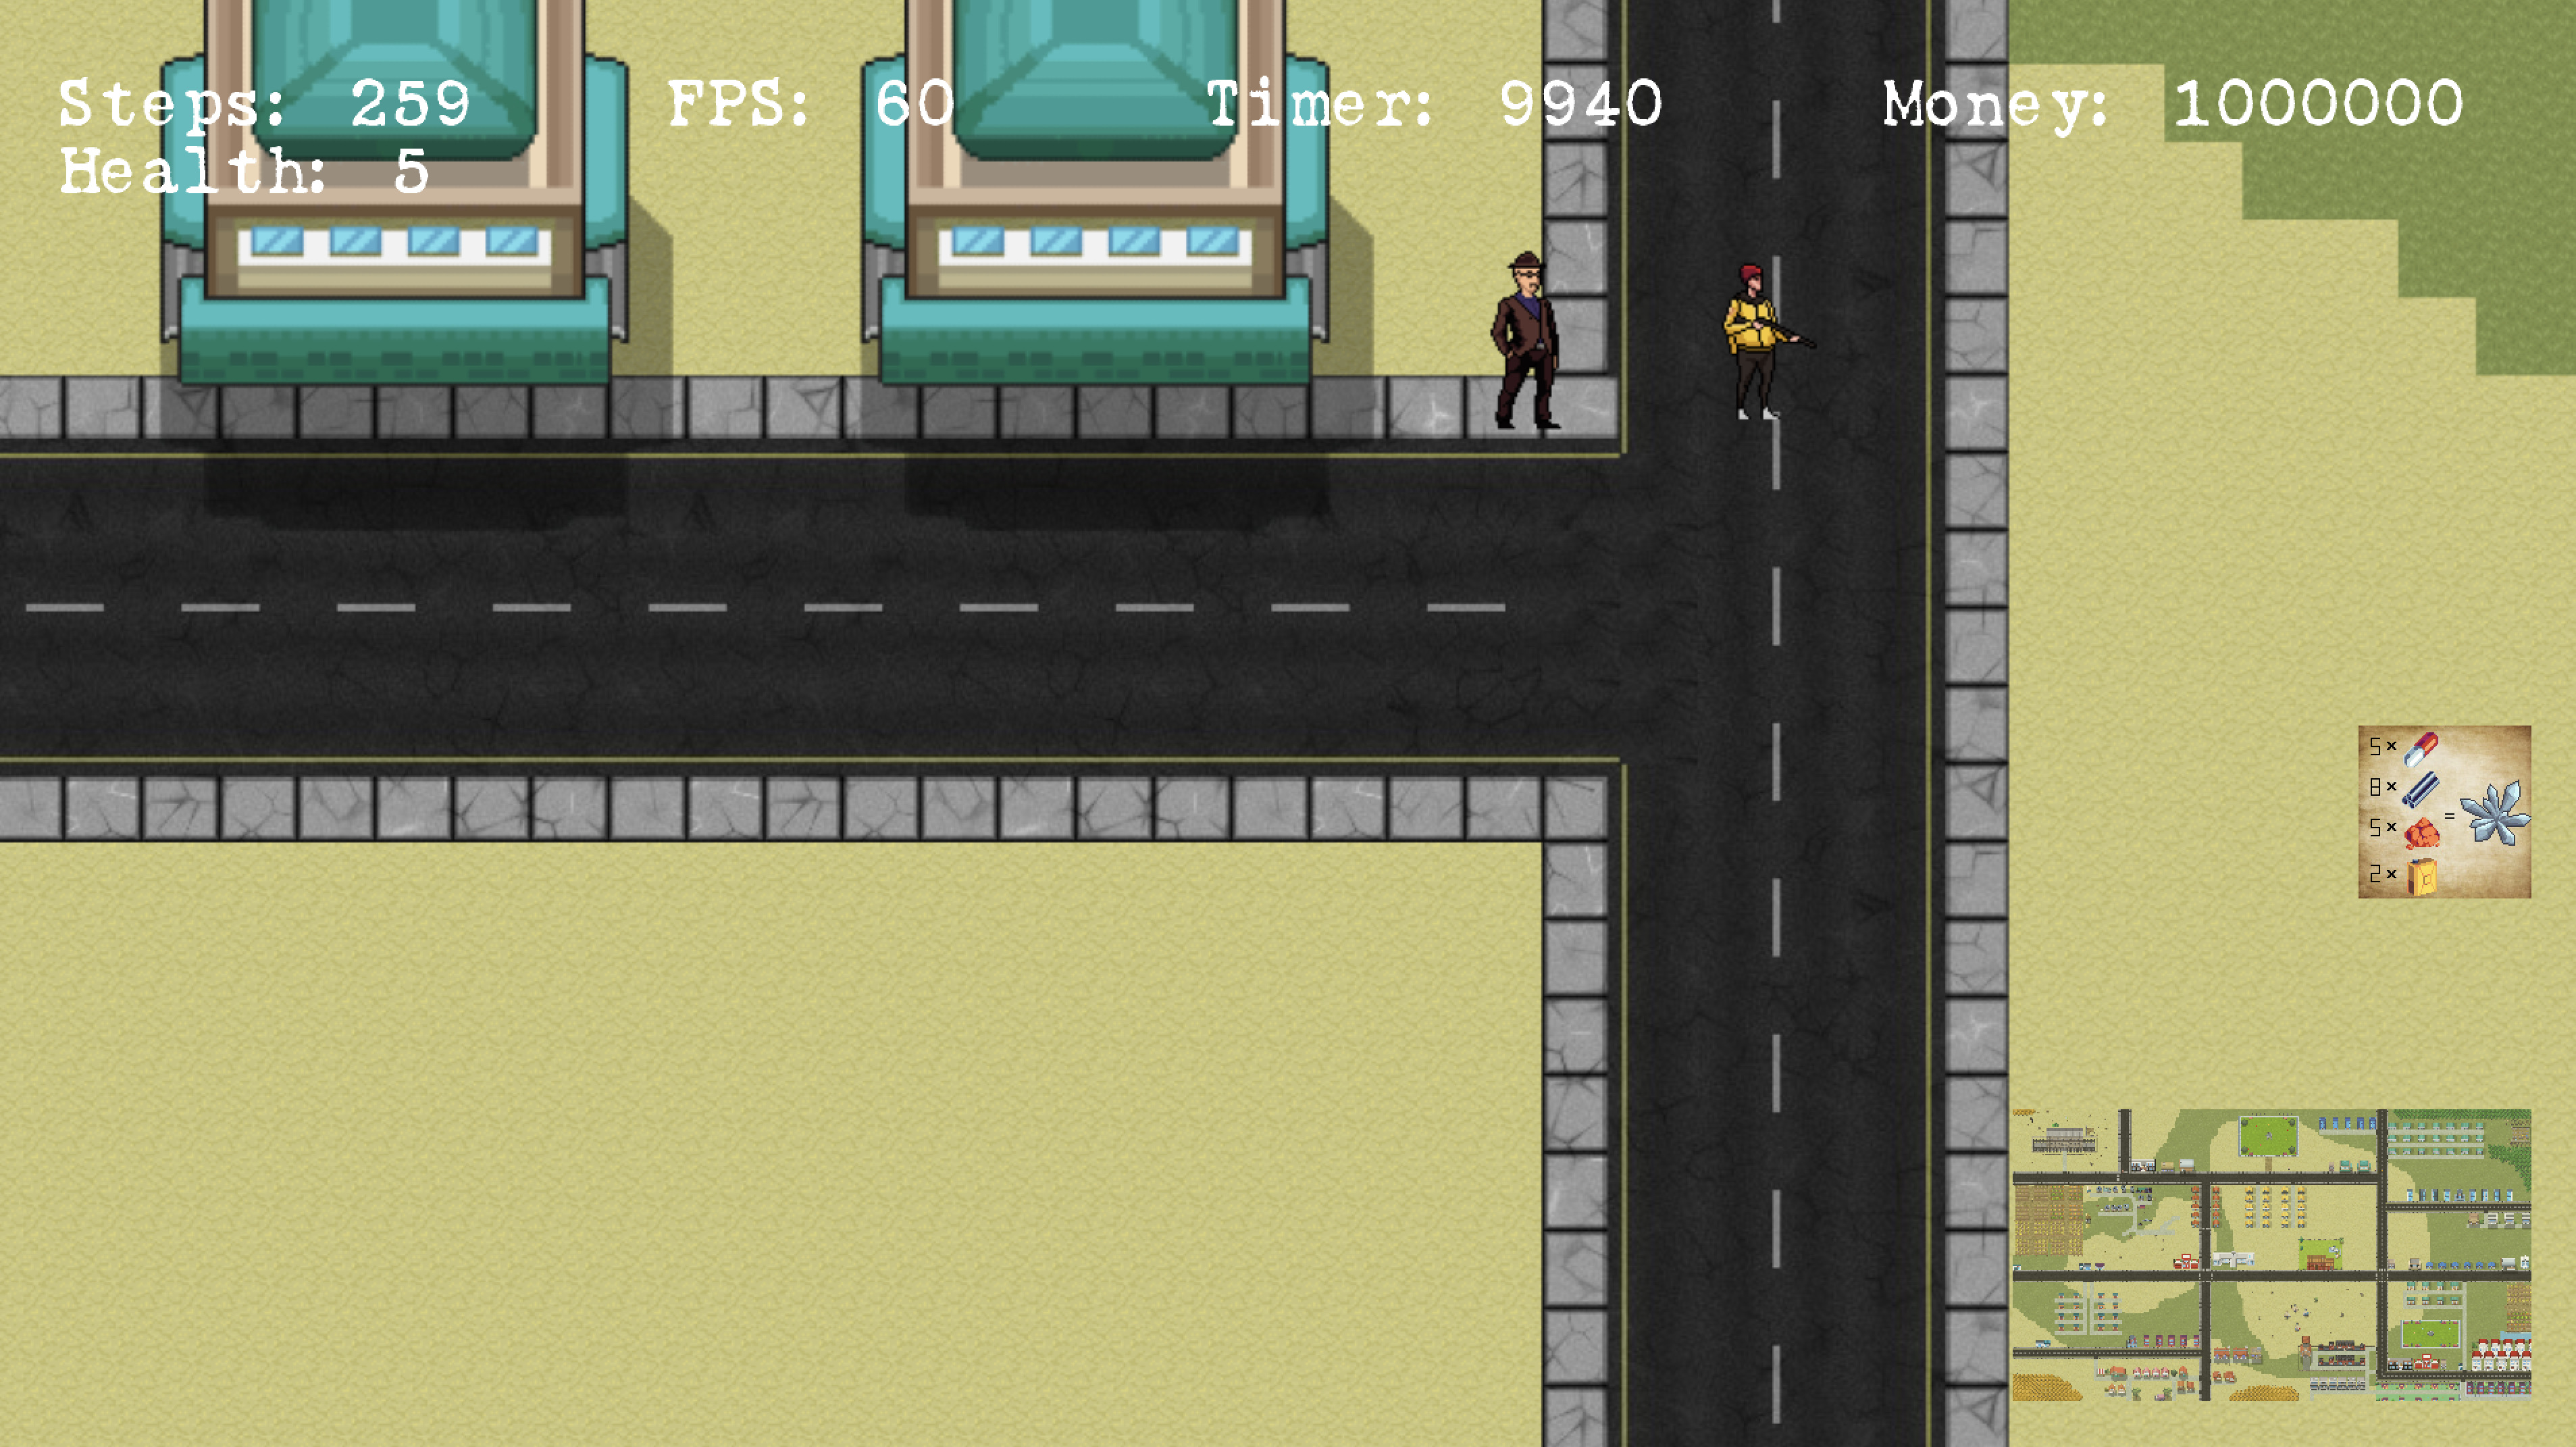
\includegraphics[width=0.85\textwidth]{./figures/InGameScreenBeispiel}
    \caption{Beispiel für Kameraperspektive mit HUD-Elementen (Farben und Icons werden noch angepasst)}
    \label{fig:figure}
\end{figure}\\
Dabei gibt es folgende HUD-Elemente:\\
\begin{itemize}
    \item \textbf{Minimap} \\
    Die Minimap ist ein von der Position der Spieler abhängiger Ausschnitt der Karte.
    Sie dient zur Orientierung und besseren Gefahren- und Fluchtwegerkennung der Spieler.
    \item \textbf{Wanted Status} \\
    Zeigt den Spielern an, wie aktiv die Polizei gerade nach ihnen fahndet.
    \item \textbf{Money} \\
    Zeigt den Spielern wie viel Geld sie gerade besitzen.
    \item \textbf{Timer} \\
    Zeigt den Spielern wie viel Zeit sie noch übrig haben bis der Todesfall durch die Krankheit eintritt.
    \item \textbf{Health Bar} \\
    Die Lebensleiste zeigt den Spielern wie viele Lebenspunkte sie gerade haben.
    \item \textbf{Zutatenliste} \\
    Die Zutatenliste zeigt den Spielern die nötigen Zutaten für das gerade ausgewählte Rezept an, sodass die Spieler sich nicht alle Zutaten auswendig merken müssen.
\end{itemize}


\subsubsection*{Steuerung}
Die zwei Spielcharaktere werden jeweils von einem Spielenden gesteuert.
Als Eingabegeräte wird das Benutzen zweier Controller (Playstation, XBox, etc.)
oder eines Controllers und einer Tastatur empfohlen.
Beide Spieler auf derselben Tastatur ist auch möglich, für die Standardbelegung
ist dafür jedoch ein Numpad erforderlich.
Sollte dieses nicht vorhanden sein, lässt sich die Steuerung beliebig anpassen. \\

\begin{table}[h!]
    \centering
    \begin{tabular}{|l|l|l|l|}
        \hline
        \multicolumn{2}{|c|}{\textbf{Tastatur}} & \textbf{Controller} & \textbf{Funktion} \\
        \hline
        \textbf{Spieler 1} & \textbf{Spieler 2} & & \\
        \hline
        W & Arrow-Up & Left-Joystick-Up & Bewegung nach oben \\&&& Menünavigation hoch \\
        \hline
        S & Arrow-Down & Left-Joystick-Down & Bewegung nach unten \\&&& Menünavigation runter \\
        \hline
        A & Arrow-Left & Left-Joystick-Left & Bewegung nach links \\
        \hline
        D & Arrow-Right & Left-Joystick-Right & Bewegung nach rechts \\
        \hline
        F & Numpad-2 & A / Cross & Interagieren \\
        \hline
        R & Numpad-3 & Y / Triangle & ausgerüstete Waffe wechseln \\
        \hline
        SPACE & Numpad-1 & X / Square & schlagen / schießen \\
        \hline
        TAB & Numpad-6 & Start / Options & Inventar öffnen \\
        \hline
        ESC & Numpad-9 & Back / Share & Pausenmenü öffnen \\
        \hline
    \end{tabular}
    \caption{Tastenbelegungen der vom Spieler ausführbaren Aktionen}
    \label{tab:steuerung}
\end{table}

\begin{description}
    \item[Bewegung]
    Mit den in \ref{tab:steuerung} beschrieben Tasten lässt sich der Spielcharakter bewegen. \\
    Bei Nutzung der Tastatur ist zusätzlich eine diagonale Bewegung möglich, indem zwei orthogonal
    zueinander gerichtete Bewegungen parallel ausgeführt werden. \\
    Bei Nutzung eines Controllers sind Bewegungen mit beliebiger Richtung möglich.
    \item[Interagieren]
    Mit der in \ref{tab:steuerung} definierten Taste lassen sich folgende Arten von
    Interaktionen durchführen:
    \begin{itemize}
        \item \textbf{Kochen}:
        Hierbei müssen sich beide Spielfiguren in der Nähe der CookingStation befinden
        und die in \ref{tab:steuerung} definierte Taste von einem der Spieler
        gedrückt werden.
        \item \textbf{Handeln}:
        Hierbei muss sich die Spielfigur in der Nähe eines interaktiven NPCs befinden.
        \item \textbf{Verstecken}:
        Hierbei muss sich die Spielfigur in der Nähe eines Busches befinden.
        \item \textbf{Türen durchschreiten}:
        Hierbei müssen sich beide Spielfiguren in der Nähe einer Tür befinden
        und die in \ref{tab:steuerung} definierte Taste von einem der Spieler
        gedrückt werden.
    \end{itemize}
    \item[ausgerüstete Waffe wechseln]
    Mit der in \ref{tab:steuerung} definierten Taste lässt sich zwischen Fäusten
    und Schusswaffe hin und her wechseln.
    \item[schlagen / schießen]
    Mit der in \ref{tab:steuerung} definierten Taste lässt sich die ausgerüstete Waffe
    anwenden, der Spielcharakter führt also einen Schlag bzw. einen Schuss aus.
    \item[Inventar öffnen]
    Mit der in \ref{tab:steuerung} definierten Taste lässt sich das Inventar-Fenster
    öffnen.
    \item[Pausenmenü]
    Mit der in \ref{tab:steuerung} definierten Taste lässt sich das Pausenmenü
    öffnen.
\end{description}

    \newpage
    \subsection{Menü-Struktur}\label{subsec:menu-struktur}

Im folgenden Abschnitt werden die einzelnen Menüs behandelt und erklärt. Vorab eine ausführliche Übersicht der Menü-Struktur:\\

\begin{figure}[H]
    \centering
    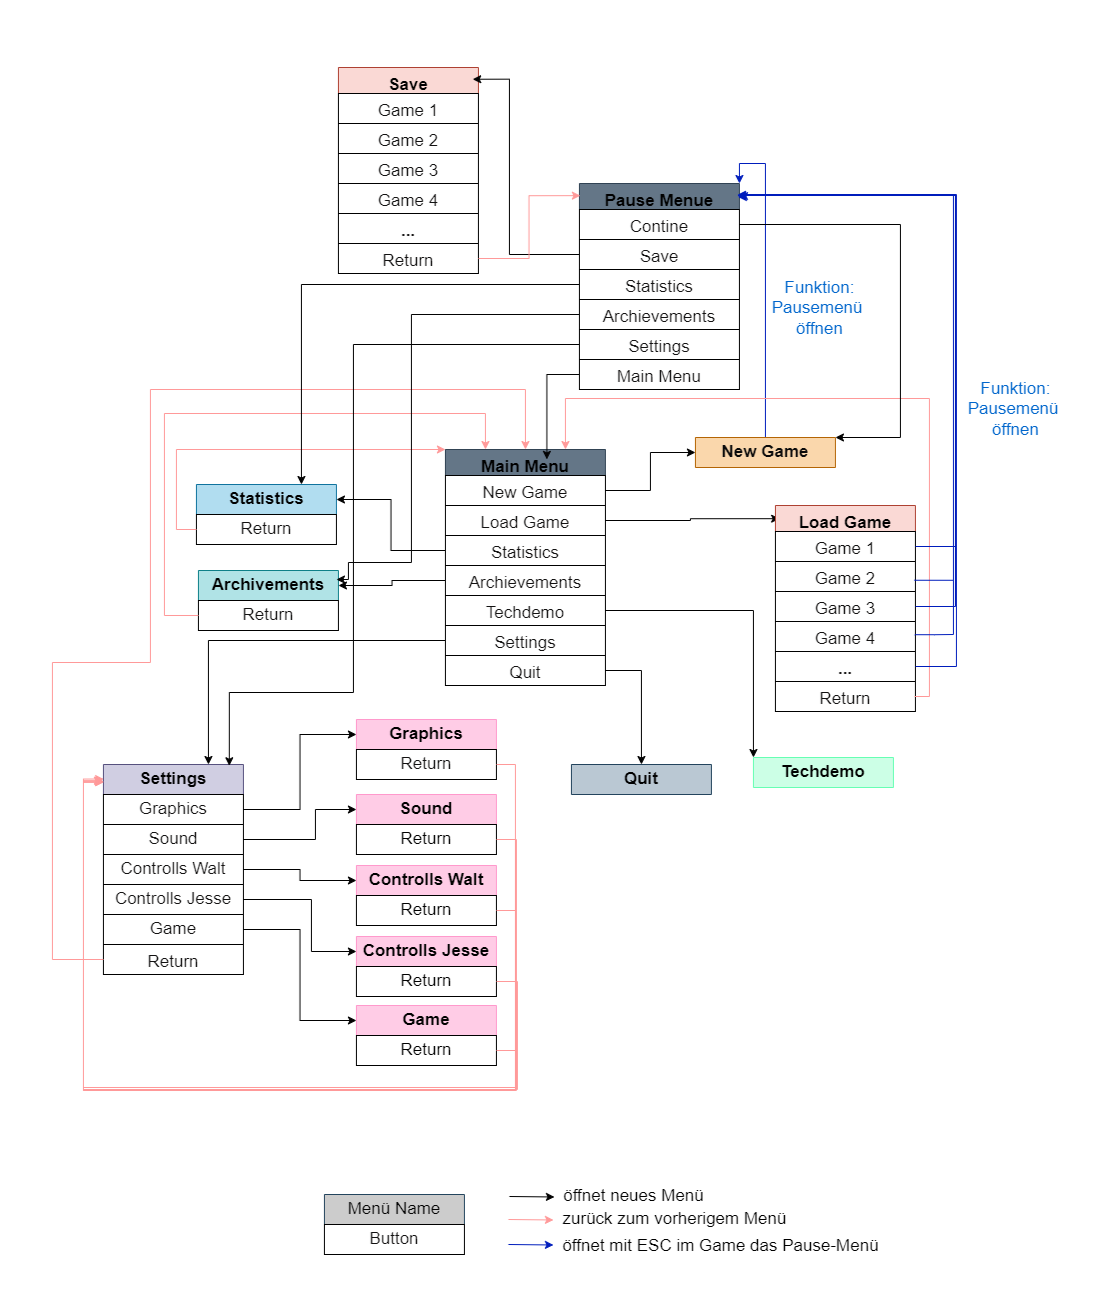
\includegraphics[width=1.0\textwidth]{figures/menuStructure}
    \caption{Menü-Struktur mit Legende}
    \label{fig:menuStructure}
\end{figure}

Nach dem Starten des Spiels wird das \textbf{Hauptmenü} mit folgenden Buttons angezeigt (Steuerung erfolgt über die Pfeiltasten oder die Maus):

\begin{itemize}
    \item \textbf{New Game:} startet ein neues Spiel mit einem neuen Speicherstand
    \item \textbf{Load Game:} Zeigt alle vorhanden Spielstände an und lädt den ausgewählten Spielstand
    \item \textbf{Statistics:} Zeigt eine Übersicht von allen vorhanden Statistiken an
    \item \textbf{Achievements:} Zeigt alle möglichen Achievements an, wie diese erreicht werden können und welche schon erreicht wurden
    \item \textbf{Settings:} Hier sind Einstellungen bezüglich des Sound, der Grafik und der Steuerung möglich: \newline
    - Controls Walt: Tastenbelegungen für Spieler1 personalisieren \newline
    - Controls Jesse: Tastenbelegungen für Spieler2 personalisieren \newline
    - Sound: Lautstärkeslider für Hintergrundmusik/Soundeffekte \newline
    - Grafik: Auswählen von Bildschirmauflösungspresets \newline
    - Game: Schwierigkeitsstufe: Leicht/Mittel/Schwierig
    \item \textbf{Quit:} Beendet das Spiel
\end{itemize}
Durch Drücken von [ESC] öffnet sich während des Spiels ein \textbf{Pausemenü}.

\begin{itemize}
    \item \textbf{Continue:} setzt das Spiel fort
    \item \textbf{Save:} Speichert den aktuellen Spielstand unter dem ausgewählten Slot
    \item  \textbf{Statistics:} Zeigt eine Übersicht von allen vorhanden Statistiken an
    \item  \textbf{Achievements:} Zeigt alle möglichen Achievements an, wie diese erreicht werden können und welche schon erreicht wurden
    \item \textbf{Settings:} Hier sind Einstellungen bezüglich des Sound, der Grafik und der Steuerung möglich: \newline
    - Controls Walt: Tastenbelegungen für Spieler1 personalisieren \newline
    - Controls Jesse: Tastenbelegungen für Spieler2 personalisieren \newline
    - Sound: Lautstärkeslider für Hintergrundmusik/Soundeffekte \newline
    - Grafik: Auswählen von Bildschirmauflösungspresets \newline
    - Game: Schwierigkeitsstufe: Leicht/Mittel/Schwierig
    \item \textbf{Main Menu:} öffnet das Hauptmenü
\end{itemize}
\newpage


    \newpage
    \section{Technische Merkmale}\label{sec:technische-merkmale}
    In diesem Abschnitt werden einerseits die verwendeten oder vorraussichtlich benötigten Technologien für die Erstellung Spiels und andererseits die Mindestvoraussetzungen, die benötigt werden um das Spiel laufen zu lassen, beschrieben.\\
    \subsection{Verwendete Technologien}\label{subsec:verwendete-technologien}

\begin{itemize}
    \item \textbf{Programmiersprache, Framework und Bibliotheken:} \\
    Microsoft C\# 12, .NET SDK 8, Monogame 3.8.2, LaTeX
    \item \textbf{IDEs und Plugins:} \\
    Rider mit MonoGame Plugin, IntelliJ IDEA Ultimate mit TeXiFy Plugin, Overleaf
    \item \textbf{Tools:} \\
    JetBrains Resharper, Jenkins, Sonar Cube, Gitea, GitHub Copilot, ChatGPT 4o
    \item \textbf{Asset Bearbeitung:} \\
    Adobe Photoshop, Inkscape, Gimp, Audacity
    \item \textbf{Kommunikation:} \\
    Discord, Mattermost
\end{itemize}
    \subsection{Mindestvoraussetzungen}\label{subsec:mindestvoraussetzungen}

\begin{itemize}
    \item \textbf{Betriebssystem:} \\
    Windows 10 (x64) - GNU/Linux (Ubuntu 22.04 LTS)
    \item \textbf{CPU:} \\
    Quad-Core Prozessor mit mindestens 2.0 GHz
    \item \textbf{Arbeitsspeicher:} \\
    8GB
    \item \textbf{GPU:} \\
    Grafikkarte mit mindestens ShaderModel 2.0
    \item \textbf{Bildschirmauflösung:} \\
    1920 x 1080
    \item \textbf{Framework:} \\
    .NET 8.0
    \item \textbf{Eingabegeräte:} \\
    Tastatur und Maus
\end{itemize}


    \newpage
    \section{Spiellogik}\label{sec:spiellogik}
    Dieses Kapitel setzt sich aus den fünf für die Spiellogik elementaren Teilen zusammen:\newline den Aktionen, den Spielobjekten, der Spielstruktur und den Statistiken und Achievements.
    \subsection{Optionen und Aktionen}\label{subsec:optionen-und-aktionen}

Im folgenden Abschnitt werden die Aktionen und Optionen, die der Spieler im Spiel verwenden kann, aufgelistet und beschrieben.\\



\let\origclearpage\clearpage
\renewcommand{\clearpage}{\relax}

\newgeometry{top=2.5cm, bottom=2.5cm, left=1.5cm, right=1.5cm}

\begin{longtable}{|p{1.6cm}|p{1.9cm}|p{5.5cm}|p{3.2cm}|p{4.2cm}|}
    \hline
    \rowcolor{gray!30}
    \textbf{ID / Name} & \textbf{Akteure} & \textbf{Ereigniseinfluss} & \textbf{Anfangsbedingungen} & \textbf{Abschlussbedingun- gen} \\
    \hline
    \endfirsthead

    \hline
    \rowcolor{gray!30}
    \textbf{ID / Name} & \textbf{Akteure} & \textbf{Ereigniseinfluss} & \textbf{Anfangsbedingungen} & \textbf{Abschlussbedingun- gen} \\
    \hline
    \endhead

    % Inhalt der Tabelle
    ID01: Laufen & Spieler, Polizei KI, NPC KI&
    1. Spieler drückt Taste (oben, unten, rechts, links / w, a, s, d) \newline
    2. Spielfigur bewegt sich in die entsprechende Richtung &
    Spielfigur befindet sich auf der Map &
    Spielfigur befindet sich weiter rechts/links/ oben/unten auf der Map \\
    \hline
    ID02: mit Tür interagieren & Spieler &
    1. beide Spielfiguren befinden sich in unmittelbarer Nähe einer begehbaren Tür \newline
    2. ein Spieler drückt die Interagieren-Taste\newline
    3. Tür öffnet sich und ein weiterer Teil der Map ist begehbar &
    beide Spielfiguren befinden sich in der Nähe einer geschlossenen Tür &
    die Spielfiguren befinden sich in der Nähe einer offenen Tür\\
    \hline
    ID03: schießen & Spieler, Kartell KI &
    1. Spieler drückt Taste \newline
    2. Spielfigur schiesst in die die Richtung in die sie schaut \newline
    3. Jeder NPC (ausser Verkäufer) und Mülleimer, der im Sichtkegel ist erhält schaden (verringert HP) &
    Spielfigur muss eine Waffe ausgewählt haben &
    Jede Spielfigur, die im Sichtkegel ist hat schaden erhalten (verringerte HP)
    ODER Mülleimer fällt um und dropt manchmal ein Item \\
    \hline
    ID04: schlagen & Spieler, Kartell KI &
    1. Spieler drückt Taste \newline
    2. Spielfigur führt Schlag aus \newline
    3. Mülleimer/Gegner in unmittelbarem Umfeld kann Schaden nehmen \newline
    Gegner verliert HP \newline
    ODER\newline
    Mülleimer fällt um und dropt manchmal ein Item&
    Spielfigur hat keine Waffe ausgewählt &
    Mülleimer ist liegt auf dem Boden ggf. ein Item daneben \newline
    ODER\newline
    Gegner/Spielfigur hat weniger HP \\
    \hline
    ID05: kochen & Spieler &
    1. Spieler drückt die interagieren Taste, während beide Spielfiguren sich in der Nähe einer Crafting Station befindet \newline
    2. Spieler wählt Rezep aus, welches zubereitet werden soll.
     Ein Minispiel startet, was erfolgreich beendet werden muss um die Drogen herzustellen.
     In diesem werden zufällig verschiedene Buttons in verschiedenen Farben auf dem Bildschirm angezeigt, 
     die der Spieler mit der zugehörigen Farbe dann in einer gewissen Zeit drücken muss. 
     Wenn die Spieler zu oft zu langsam sind oder die falsche Taste drücken schlägt die Herstellung fehl 
     und das Minispiel endet und die zur Herstellung verwendeten Materialien werden zerstört. &

    Beide Spielfiguren befinden sich in der Nähe der Crafting Station &
    Weniger Ressourcen und falls das Kochen erfolgreich war mehr Drogen im Inventar \\
    \hline
    ID06: mit Käufer/ Verkäufer handeln & Spieler &
    1. Spieler drückt interagieren Taste, während die Spielfigur sich in der Nähe eines interaktiven NPC aufhält \newline
    2. je nach NPC: \newline
    - Verkäufer: es öffnet sich ein Dialog-Feld und zeigt die zu kaufenden Gegenstände an \newline
    - Käufer: bietet bestimmte Menge Geld für bestimmte Menge Drogen (unterschiedlich je Käufer), Spieler kann das Angbot annehmen oder ablehnen &
    Spielfigur befindet sich in unmittelbarer Nähe von einem interaktiven NPC &
    Bei Kauf: Mehr Ressourcen und weniger Geld \newline
    ODER \newline
    Bei Verkauf: Mehr Geld und weniger Drogen \newline
    ODER \newline
    Man nimmt das Angebot nicht an/ kauft nichts, man hat also gleich viel Ressourcen und Geld wie davor\\
    \hline
    ID07: Items aufnehmen & Spieler &
    1. Spielfigur befindet sich auf einem Item \newline
    2. Item verschwindet von Map und wird im Inventar abgelegt &
    Spielfigur befindet sich direkt vor dem Item &
    Item befindet sich im Inventar der Spielfigur und ist von der Map verschwunden \\
    \hline
    ID08: Polizist verfolgt Spielfigur & Polizei KI&
    1. Polizist bemerkt verdächtiges Verhalten(z.B. Verkauf von Drogen, schießen, \dots) innerhalb seines Radars \newline
    2. Polizist identifiziert Spieler \newline
    3. Polizist verfolgt Spieler, solange dieser in seinem Sichtfeld/Radar ist  &
    Spielfigur befindet sich im Radar des Polizisten und tut etwas Verdächtiges &
    Spielfigur konnte vor Polizei fliehen oder sich verstecken \newline
    ODER\newline
    Polizei nimmt Spielfigur gefangen und sie kommt ins Gefängnis \\
    \hline
    ID09: verstecken & Spieler &
    1. Spielfigur befindet sich in der Nähe eines Busches\newline
    2. Spieler drückt Taste\newline
    - wenn sich die Spielfigur innerhalb des Radius der Polizei befindet ist verstecken nicht möglich, da die Polizei das sonst sieht
    - außerhalb des Radius der Polizei kann sich die Spielfigur in dem Busch verstecken und ist für die Polizei nicht auffindbar &
    Spielfigur befindet sich neben einem Busch und außerhalb des Radius der Polizei &
    Spielfigur befindet sich in dem Busch und ist für Polizei nicht sichtbar \\
    \hline
    ID10: Waffe wechseln & Spieler &
    1. Spieler drückt Taste zum Waffe wechseln \newline
    2. Waffe wird gewechselt &
    Spielfigur hat Pistole nicht ausgewählt\newline
    ODER\newline
    Spielfigur hat Pistole ausgewählt &

    Spielfigur hat Pistole ausgewählt wenn vorher nicht ausgewählt \newline
    ODER\newline
    Spielfigur hat nicht die Pistole ausgewählt, wenn vorher ausgewählt  \\
    \hline
\end{longtable}

\let\clearpage\origclearpage
\restoregeometry



    \newpage
    \newgeometry{top=2.5cm, bottom=2.5cm, left=1.5cm, right=1.5cm}
\subsection{Spielobjekte}\label{subsec:spielobjekte}

\begin{tabular}{|m{1.5cm}|m{13cm}|m{2.5cm}|}
    \hline
    \textbf{Name} & \textbf{Beschreibung} & \textbf{Art} \\
    \hline
    Walter/ \newline Jesse &
    Diese beiden Spielfiguren sind die von den Spielenden kontrollierten Objekte.
    Spielfigur 1 ,,Walt'' wird von Spieler 1 gesteuert und auf der Map bewegt, Spielfigur 2 ,,Jesse'' von Spieler 2. Sie sind durch die Aktionen und Interaktionen mit anderen Spielobjekten schon hinreichend definiert. Da beide die gleichen Eigenschaften haben zählen sie als ein Objekt.\newline
    \textbf{Aktionen}: Laufen ID01, Mit Tür interagieren ID02, Schiessen ID03, Schlagen ID04, Kochen ID05, Interagieren ID06, Items aufnehmen ID07, Verstecken ID09, Waffe wechseln ID10 \newline
    \textbf{Eigenschaften:} Health, Money, Inventory, Wanted Level, Bewegungsgeschwindigkeit ist ca 20\% höher als die der Polizei um eine Chance zum Entkommen zu haben.

    & kontrollierbar \newline
    kollidierend \newline
    beweglich \\

    \hline
    Polizei &
    Polizei ist einer der beiden Gegnertypen im Spiel, sie werden durch eine KI gesteuert.
    Sie laufen auf der Map herum, vor allem dort wo viele NPCs sind.
    Das Polizeiaufgebot hängt vom aktuellen Fahndungslevel ab, heißt je gesuchter Walt und Jesse gerade sind, desto mehr Polizisten verfolgen sie.
    Ein einzelner Polizist hat ein kegelförmiges Sichtfeld.
    Führen Walt oder Jesse in diesem Bereich eine verdächtige Aktion aus (dazu gehören Drogen verkaufen, Zutaten einkaufen, im Busch verstecken, Kartell angreifen und Polizei angreifen), dann wird der Polizist alerted und das globale Fahndungslevel steigt.
    Schaffen es Walt und Jesse für einen gewissen Zeitraum außerhalb des Sichtfelds jeglicher Beamten zu bleiben, so wird das Fahndungslevel wieder auf 0 gesetzt.
    Während das Fahndungslevel größer 0 ist verfolgen die Polizisten Walt und Jesse.
    Schafft es ein Polizist nah genug an Walt oder Jesse heranzulaufen gilt das als festnehmen und der globale Timer wird verkürzt (simuliert Gefängnis).
    Walt und Jesse können also durch Wegrennen entkommen.
    Sie können aber auch durch schlagen und schießen Polizisten ausschalten. &
    kontrollierbar (durch KI), kollidierend, beweglich\\
    \hline

    \hline
    Kartell &
    Kartellmitglieder sind eine der beiden Gegnertypen im Spiel.
    Sie konkurrieren mit Walt und Jesse im Drogengeschäft und sind ihnen deshalb feindlich gesinnt
    Sie laufen alleine oder in Gruppen durch ihre Reviere (nicht die ganze Map).
    Sie haben ein kegelförmiges Sichtfeld.
    Befindet sich Walt oder Jesse in diesem Sichtfeld greift das Kartellmitglied sofort an.
    Dabei kommen Fäuste und Waffen zum Einsatz (abhängig von Schwierigkeitsstufe)
    Um diesen Angriff zu beenden, können Walt und Jesse das Kartellmitglied entweder umbringen oder das Revier des Kartells verlassen.&
    kollidierend, beweglich\\
    \hline

    \hline
    NPC &
    Verkäufer NPCs sind Bewohner der Stadt, die überall auf der Map anzutreffen sind.
    Sie können stationär an einem Punkt stehen bleiben aber auch durch die KI gesteuert über die Map laufen und sich zu Orten mit wenig Polizeipräsenz bewegen.
    Walt und Jesse können ihnen Drogen verkaufen.
    Das Handeln mit NPCs in Revieren des Kartells ist meistens lukrativer. &
    kontrollierbar (durch KI), kollidierend, beweglich\\
    \hline

\end{tabular}
\newpage
\noindent
\begin{tabular}{|m{1.8cm}|m{12.7cm}|m{2.5cm}|}
    \hline
    Verkäufer / Shop &
    Verkäufer/Shop sind Bewohner/Gebäude der Stadt, die auf der Map anzutreffen sind.
    Walt und Jesse können bei ihnen Zutaten kaufen.
    In den Shops können Walt und Jesse andere Items kaufen als bei den Verkäufern. &
    kontrollierbar (durch KI), kollidierend, beweglich\\
    \hline

    \hline
    Crafting Station &
    Wenn die Spielfiguren sich in der Nähe der Crafting Station befinden, können sie die Aktion kochen (ID06) ausführen.
    Es öffnet sich ein Dialogfeld, bei dem man auswählen kann, welches Rezept gekocht werden soll. Außerdem wird eine
    Übersicht mit allen vorhandenen Zutaten angezeigt. Danach muss ein Minispiel erfolgreich beendet werden, damit
    die Droge auch wirklich hergestellt wird. Ansonsten gehen die Zutaten verloren. Im Verlaufe des Spiels können die Spieler die Crafting Station upgraden,
     um neue Rezepte freizuschalten und somit noch Wertvollere Drogen herstellen zu können&
    auswählbar, kollidierend\\
    \hline

    \hline
    Busch &
    Die Spielfiguren haben während des Spiels die Möglichkeit mit Aktion ID09 sich in einem Busch zu verstecken.
    Die Spielfigur verschwindet von der Map und ist auch für die Polizei unsichtbar. Das gilt allerdings nur,
    wenn die Spielfigur nicht gerade von der Polizei verfolgt wurde, also sich nicht im Radius eines Polizisten befindet.
    Anderenfalls sieht der Polizist wie die Spielfigur sich versteckt und kann ihn trozdem fangen und festnehmen. &
    auswählbar\\
    \hline

    \hline
    Mülleimer &
    Auf der Map befinden sich Mülleimer, die vom Spieler mit einem Schlag (ID04) umgeworfen werden können. Manchmal wird dann eine Zutat gedropt.
    Nach einer bestimmten Zeit verschwindet der umgeworfene Mülleimer und spawnt neu und kann erneut umgeschmissen werden. &
    kontrollierbar, kollidierend\\
    \hline

    \hline
    Tür &
    Manche Türen im Spiel können mit Aktion ID02 geöffnet werden, und ermöglichen dadurch den Zugang zu einem weiteren Teil der Map (z.B. Haus). &
    auswählbar, kollidierend, kontrollierbar\\
    \hline


    %\caption{Spielobjekte}
    %\label{tab:spielobjekte}

\end{tabular}

\newgeometry{top=2.5cm, bottom=2.5cm, left=2.5cm, right=2.5cm}
    \newpage
    \subsection{Spielstruktur}\label{subsec:spielstruktur}


"`Breaking Worse"' ist ein Spiel, in dem die Spielenden in die Welt der Drogen eintauchen und sich mit Aktivitäten beschäftigen, die von der Herstellung und dem Kochen bis hin zur Verteilung und dem Verkauf reichen. Die Spielfiguren stehen vor einer ernsten gesundheitlichen Situation, die sie dazu zwingt, ein teures Heilmittel zu kaufen, um die tödliche Krankheit zu besiegen, bevor die Zeit abläuft.

\subsubsection{Spielphasen}

\paragraph{Early-Game} Die Spielfiguren beginnen in einer Küche,
 in der ihnen verschiedene Werkzeuge und Rezepte zur Verfügung stehen.
 Um mit dem Kochen zu beginnen, müssen sie jedoch nach draußen gehen,
 um auf der Karte wichtige Zutaten zu sammeln. Sobald sie diese Zutaten eingesammelt haben, 
 kehren sie in die Küche zurück, um mit dem Herstellen zu beginnen.

\paragraph{Mid-Game} Nach dem Fertigstellen der Kreationen können die Spieler:innen erneut die Karte erkunden, 
um ihre Produkte zu verkaufen. Dies geschieht durch die Interaktion mit NPCs, 
die jeweils bestimmte Bedürfnisse und Mengen haben. 
Dabei müssen die Spieler:innen aufmerksam bleiben, denn die Stadt wird streng von der Polizei überwacht. 
Werden sie erwischt, drohen ihnen Zeit- und Geldstrafen.

\paragraph{Late-Game} Während die Spielfiguren weiter herstellen und verkaufen,
steigt ihr Verdachtslevel, was erhöhte Vorsicht erfordert und das Risiko höherer Zeitstrafen
durch Gefängnisaufenthalte mit sich bringt. Mit ausreichend Geld können sie Werkzeuge aufrüsten
und neue Rezepte freischalten, um stärkere Substanzen herzustellen. Das ultimative Ziel des Spiels ist es,
den finalen Gegenstand zu erwerben: das Heilmittel gegen Krebs,
um die Krankheit endgültig zu besiegen.

\subsubsection{Dynamik des Spiels}

Einige Gebiete der Karte werden vom rivalisierenden Kartell besetzt, das nicht zögert, 
auf die Spielfiguren zu schießen, wenn diese ihren Weg kreuzen. 
Jeder Schaden, den die Spieler:innen von ihnen erleiden, 
verringert die gemeinsame Gesundheitsanzeige, 
die entweder mit der Zeit regeneriert oder gegen eine Gebühr im Krankenhaus wiederhergestellt werden kann.
 Ein tödlicher Angriff durch das Kartell lässt die Spielfiguren im Krankenhaus mit geringer Gesundheit und einer erheblichen Geldstrafe wieder erscheinen.

Die Polizeialarmbereitschaft wird direkt durch das Aktivitätsniveau der Spielfiguren beeinflusst.
Die Spielenden haben die Wahl, entweder mit Gewalt gegen die Polizei vorzugehen,
was deren Wachsamkeit und die Schwierigkeit erhöht,
oder sich vorsichtig zu verhalten,
indem sie zum Beispiel die Spielfiguren in Büschen verstecken wenn diese verfolgt werden,
um Konfrontationen zu vermeiden.

\subsubsection{Mögliche Spielmodi und Strategie}

Das Spiel bietet 3 Schwierigkeitsgrade, je nach dem gibt es weniger Zeit, schneller steigendes Fahndungslevel niedrigere Verkaufspreise und längere Gefängnisstrafe.

Zusammenfassend erlaubt es "`Breaking Worse"' den Spielenden, ihre Herangehensweise und Strategie 
flexibel zu gestalten und durch taktisches Verhalten langfristig zu profitieren.


    \subsection{Statistiken}\label{subsec:statistiken}

\noindent Während des Spielens werden Statistiken über verschiedene Metriken für die Spielfiguren erstellt. Diese können im Statistik Menü angeschaut werden.

\vspace{1cm}

\begin{itemize}
    \item Total of recipes unlocked \newline - Die Anzahl der freigeschalteten Rezepte.
    \item Total of times dealt (drug sell)\newline - Die Anzahl der Drogenverkäufe.
    \item Total of successful cooking\newline - Die Menge der gekochten Drogen.
    \item Total damage taken\newline - Die Anzahl des erlittenen Schadens.
    \item Total received money\newline - Die Summe des erhaltenen Geldes.
    \item Total of steps\newline - Die Anzahl der gelaufenen Schritte der beiden Spielfiguren.
    \item Time since last arrest\newline - Die Zeit seit der letzten Gefangennahme durch die Polizei.
    \item Total of cartel members killed\newline - Die Anzahl der getöteten Kartel NPCs.
    \item Highest wanted level\newline - Das höchste erreichte Wanted Level.
    \item Total hospital visits \newline - Die Anzahl der Krankenhausbesuche.
\end{itemize}
    \newpage
    \subsection{Achievements}\label{subsec:achievements}

Im Spiel können durch erreichen von gewissen Merkmalen, z.B. eine gewisse Menge an Geld verdient oder das erste Mal im Gefängnis sein, Achievements freigeschaltet werden. Diese erscheinen bis zum Freischalten nur als Icon mit Fragezeichen im Achievements Menü, nach dem Freischalten mit einem eigenen Bild.
\vspace{0.5cm} 
\begin{center}
    \begin{tabular}{ccccc}
        
\includegraphics[width=1.5cm]{./figures/Question.png} & 
        
\includegraphics[width=1.5cm]{./figures/Weed.png} & 
        
\includegraphics[width=1.5cm]{./figures/Money.png} & 
        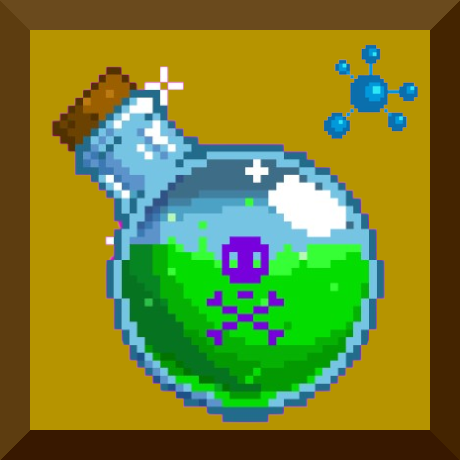
\includegraphics[width=1.5cm]{./figures/Potion.png} & 
        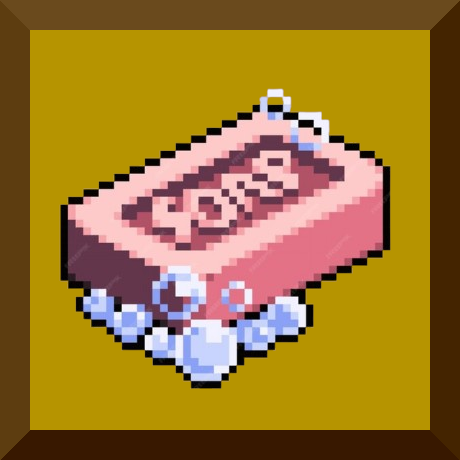
\includegraphics[width=1.5cm]{./figures/Soap.png} \\
    \end{tabular}
\end{center}
\begin{center}
    Abbildung 4: Beispiele für achievement Icons, locked und unlocked.
\end{center}

\vspace{1.5cm} 

\textbf{Zu erreichende Achievements und die Bedingungen zum Freischalten:}
\begin{itemize}
    \item \textbf{New Sprout in Town}: Craft and sell for the first time \newline - Nach dem ersten Verkaufen.
    \item \textbf{We Bankin’}: Make your first Million\$ \newline - Nach erreichen eines Geldbestandes von 1000000 Einheiten.
    \item \textbf{Walter Who?}: Unlock all the recipes \newline - Nach freischalten aller Rezepte.
    \item \textbf{Don’t Drop the Soap}: Land for the first time in jail \newline - Nach der ersten Gefangennahme durch die Polizei.
    \item \textbf{So Blue…}: Deliver 1.000kg of pure meth \newline - Nach dem Herstellen und Verkaufen von 1000 Einheiten Drogen.
    \item \textbf{Scavenger}: Find 10 different ingredients in the map \newline - Nach dem Finden von mindestens 10 verschiedenen Zutaten.
    \item \textbf{Most Wanted}: Reach a 100\% wanted level \newline - Nach dem erreichen eines Wanted Levels von 100\%.
    \item \textbf{Sharp Shooter}: Take down 100 cartel members \newline - Nach dem töten von 100 Cartel NPCs.
    \item \textbf{Chill Spot}: Successfully hide in 10 bushes \newline - Nach dem Verstecken in mindestens 10 Gebüschen.
    \item \textbf{Cancer Free}: Complete the game by finally healing from your cancer \newline - Nach dem Kaufen der heilenden Medizin und Gewinnen des Spiels.
\end{itemize}

    \newpage
    \section{Screenplay}\label{sec:screenplay}
    
Tauche ein in die Welt des 50-jährigen Walter White, der mit seiner Frau und seinem Sohn in Albuquerque, New Mexico lebt. Da sein Gehalt als Chemielehrer zum Ernähren seiner Familie nicht ausreicht, muss er nebenbei noch bei einer Autowaschanlage unter schlimmsten Bedingungen für einen Hungerlohn arbeiten, um sich über Wasser zu halten und seiner Familie ein gutes Leben zu ermöglichen. Dieses verläuft auch ganz normal, bis ihn eines Tages ein Schicksalsschlag trifft. Die Diagnose - Lungenkrebs im Endstadium, unheilbar. \newline Die Lebensverlängernden Chemotherapien würden ihn ein Vermögen kosten; Geld, was Walter unmöglich auftreiben kann. Nach einem anstrengenden Tag in der Waschstraße und unzähligen Schikanen seines Chefs platzt Walter der Kragen - er kündigt. Ohne zu wissen wie es nun weitergehen soll, begleitet er seinen Schwager, der beim DEA arbeitet, auf eine Drogenrazzia, wo er unerwartet einen alten bekannten wiedertrifft - seinen ehemaligen Schüler Jesse, der auf die schiefe Bahn gerutscht ist und nun mit Drogen handelt. Dessen Partner wurde soeben vom DEA verhaftet, er selbst konnte allerdings fliehen. Als Walter die Berge von Geld sieht, die bei der Razzia beschlagnahmt wurden, fasst er einen Entschluss: Er überzeugt Jesse mit ihm zusammen ins Drogengeschäft einzusteigen.\newline Mit Walters Expertise im Umgang mit Chemikalien und Jesses Erfahrungen im Handel mit Drogen sind Sie auf dem besten Weg sich mit der Herstellung und dem Verkauf von Methamphetaminen ein Imperium aufzubauen. Doch nun startet ein Wettlauf gegen die Zeit, denn von dieser hat Walter nicht mehr allzuviel. \newline Sie müssen stetig genug Meth produzieren und verkaufen, um Chemotherapien für Ihn bezahlen zu können, bevor seine Zeit abläuft. Im Weg steht den beiden dabei allerdings die Polizei, die die Straßen von Albuquerque aufmerksam beobachtet, sowie die ständige Bedrohung durch das Kartell, dem es gar nicht gefällt dass plötzlich ein neuer Konkurrent den Markt bedient. Um aus diesem Teufelskreis auszubrechen hat Walter nur eine Möglichkeit: genug Geld für das ultimative Heilmittel zu sparen, welches seinen Krebs endgültig besiegen würde. Schaffst du es Walter zu retten? Probiere es aus!

\end{document}
